% !TeX root = ../thuthesis-example.tex

\chapter{IoTDB 现有写入机制分析与优化总览}
本章首先介绍 Apache IoTDB 目前已有的 \emph{insertRecords} 和 \emph{insertTablet} 接口,随后介绍 \emph{insertRecords} 写入接口执行的全部流程,包括客户端侧的数据封装、RPC 层的数据序列化与反序列化、存储引擎侧写入内存表以及最终持久化的过程。最后使用 IoT Benchmark 对 \emph{insertRecords} 接口进行性能测试和分析,找出目前 \emph{insertRecords} 接口性能不如预期的原因,为本文后续设计新 \emph{insertRecords} 写入机制提供参考。
\section{IoTDB 现有写入接口}
在 \ref{sec:chap1-sec1} 和 \ref{sec:chap1-sec2} 节中,我们简要介绍了 Apache IoTDB 现有的 \emph{insertRecords} 接口和 \emph{insertTablet} 接口,以及它们运行的整体流程。在本节中我们将进一步深入讨论 \emph{insertTablet} 和 \emph{insertRecords} 接口的设计以及两者在不同场景下的适用情况。

\subsection{Apache IoTDB 写入接口形式}
目前 IoTDB 主要提供了四种原生写入接口,分别是 \emph{insertRecord}、\emph{insertRecords}、\emph{insertTablet}、\emph{insertTablets}。这四种接口中 \emph{insertRecords}、\emph{insertTablet}、\emph{insertTablets} 都是批量化的写入接口,只有 \emph{insertRecord} 一次只写入一条记录。由于批量化写入可以将写入过程中的一些固定代价均摊到多个数据点上,可以减少写入总体代价\cite{bercken2001evaluation},因此 \emph{insertRecord} 的性能远不如其他三个接口,在生产环境中也几乎没有用户使用。以 IoTDB 的 Java SDK 为例,它们的接口定义如下:
\begin{lstlisting}[language=java,frame = trBL , firstnumber = last , escapeinside={(*@}{@*)}]
  void insertRecord(
      String deviceId,
      long time,
      List<String> measurements,
      List<TSDataType> types,
      List<Object> values
      )

  void insertRecords(
      List<String> deviceIds, 
      List<Long> times, 
      List<List<String>> measurementsList, 
      List<List<TSDataType>> typesList, 
      List<List<Object>> valuesList
      )

  void insertTablet(Tablet tablet)

  void insertTablets(Map<String, Tablet> tablets)
\end{lstlisting}
其中,Tablet 是一个数据结构,代表一个设备的一批数据,其结构如下:
\begin{lstlisting}[language=java,frame = trBL , firstnumber = last , escapeinside={(*@}{@*)}]
public class Tablet {
  public String deviceId;
  private List<MeasurementSchema> schemas;
  public long[] timestamps;
  public Object[] values;
  public int rowSize;
}
\end{lstlisting}
\emph{insertRecord} 和 \emph{insertRecords} 的参数含义则如表 \ref{tabular:insert-record-params} 和表 \ref{tabular:insert-records-params} 所示,\emph{Tablet} 的成员变量含义如表 \ref{tabular:class-tablet-param} 所示。
\begin{table}
  \centering
  \caption{insertRecord 参数说明}
  \begin{tabular}{lll}
    \toprule
    参数名 &  类型 & 描述 \\
    \midrule
    deviceId & String & 数据所属的设备 ID \\
    time & long & 数据的时间戳 \\
    measurements & List<String> & 每个数据点所属的时间序列 ID 组成的列表 \\
    types & List<TSDataType> & 每个数据点所对应的数据类型 \\
    values & List<Object> & 每个数据点的数据 \\
    \bottomrule
  \end{tabular}
  \label{tabular:insert-record-params}
\end{table}

\begin{table}
  \centering
  \caption{insertRecords 参数说明}
  \begin{tabular}{lll}
    \toprule
    参数名 &  类型 & 描述 \\
    \midrule
    deviceIds & List<String> & 每行记录所属的设备 ID 组成的列表 \\
     times & List<Long> & 每行记录的时间戳组成的列表 \\
    measurementsList & List<List<String> > & 每行记录的序列 ID 列表组成的列表 \\
    typesList & List<List<TSDataType> > & 每行记录数据类型列表组成的列表 \\
    valuesList & List<List<Object> > & 每行记录值列表组成的列表 \\
    \bottomrule
  \end{tabular}
  \label{tabular:insert-records-params}
\end{table}

\begin{table}
  \centering
  \caption{Tablet 类成员变量含义说明}
  \begin{tabular}{llp{6cm}}
    \toprule
    参数名 &  类型 & 描述 \\
    \midrule
    deviceId & String & 该 Tablet 所属的设备 ID \\
    schemas & List<MeasurementSchema> & 该 Tablet 中每个测点的元数据信息 \\
    timestamps & long 类型数组 & 该 Tablet 中每一行数据的时间戳 \\
    values & Object 类型数组 & 该 Tablet 中每一个测点的数据,其中的每一个对象都代表一列数据 \\
    rowSize & int & 该 Tablet 中包含的数据行数\\
    \bottomrule
  \end{tabular}
  \label{tabular:class-tablet-param}
\end{table}

从接口形式上看,\emph{insertRecords}、\emph{insertTablet} 和 \emph{insertTablets} 其实都是在不同维度上进行批量化的写入接口:
\begin{itemize}
  \item \emph{insertRecords} 一次性可以写入多行数据,每一行数据都是任意一个设备在同一个时间戳下若干个测点的数据,不同行之间可以是不同的设备在不同时间戳下的数据。从这一点看,\emph{insertRecords} 是在多设备、多时间戳维度上进行批量化的写入接口。
  \item \emph{insertTablet} 一次写入一个 Tablet,每个 Tablet 只能包含一个设备在不同时间戳下的数据,不同设备的数据无法共享一个 Tablet。因此,\emph{insertTablet} 是对同一个设备在多时间戳维度上进行的批量化写入。
  \item \emph{insertTablets} 一次可以写入多个 Tablet,每个 Tablet 包含一个设备在不同时间戳下的数据。因此,\emph{insertTablets} 其实也是在多设备、多时间戳维度上进行批量化的写入接口。
\end{itemize}
\emph{insertRecords} 接口和 \emph{insertTablets} 接口在批量化的维度上是相同的,因此理论上使用 \emph{insertRecords} 接口的场景都可以使用 \emph{insertTablets},反之亦然。然而,由于 \emph{insertTablets} 接口要求用户先将需要写入的数据按照设备归类并封装成 Tablet 结构体,对于用户而言使用复杂度较高,\emph{insertRecords} 对数据形式的要求则更低,因此使用 \emph{insertRecords} 的用户数更多。
\subsection{不同写入接口的性能对比\label{sec:chap3-sec1-1}}
但是这两者在数据结构上有所不同。在 \emph{insertRecords} 中,属于同一个设备的数据可能会分布在不同的位置;在 \emph{insertTablets} 中,属于同一个设备的数据会被集中在同一个 Tablet 中。后一种模式能够在写入的后续处理流程中占有一些优势:数据在写入时首先进入内存表(MemTable)中,IoTDB 将同一个设备下的时间序列存储在内存表中的同一个块组(Chunk Group)中,如果同一个设备的数据都聚集在一起,那么就可以将它们一起写入到块组中,数据写入内存表的次数与 Tablet 的个数相同。而在 \emph{insertRecords} 的写入过程中,由于每一条 Record 都可能属于不同设备,因此只能一条一条 Record 地进行写入,写入内存表的次数与 Record 的数量相同,性能在某些情况下相比 \emph{insertTablets} 可能更低。

为了对比目前 \emph{insertRecords} 接口与 \emph{insertTablets} 的性能,笔者使用 IoTDB Benchmark\cite{liu2019benchmarking} 对 IoTDB 的 \emph{insertRecords} 和 \emph{insertTablets} 接口在不同的请求模式下进行测试。笔者固定单个写入请求的数据总行数为 400,调节单个请求中不同设备数,观察两种接口的性能变化\footnote{IoTDB 版本为 1.3.0,实验环境 CPU 为 I7-11700,DataNode 使用 28GB 内存,ConfigNode 2GB,硬盘为 HDD}。例如,如果一个请求中只有 1 个设备,那么一个请求中的 400 行都是该设备的数据;如果一个请求中有 10 个设备,那么请求中每个设备都各自有 40 行数据。图 \ref{fig:records-vs-tablets-throughput} 和图 \ref{fig:records-vs-tablets-latency} 分别展示了两种接口吞吐和延迟随设备数不同而出现的变化。

\begin{figure}
  \centering 
  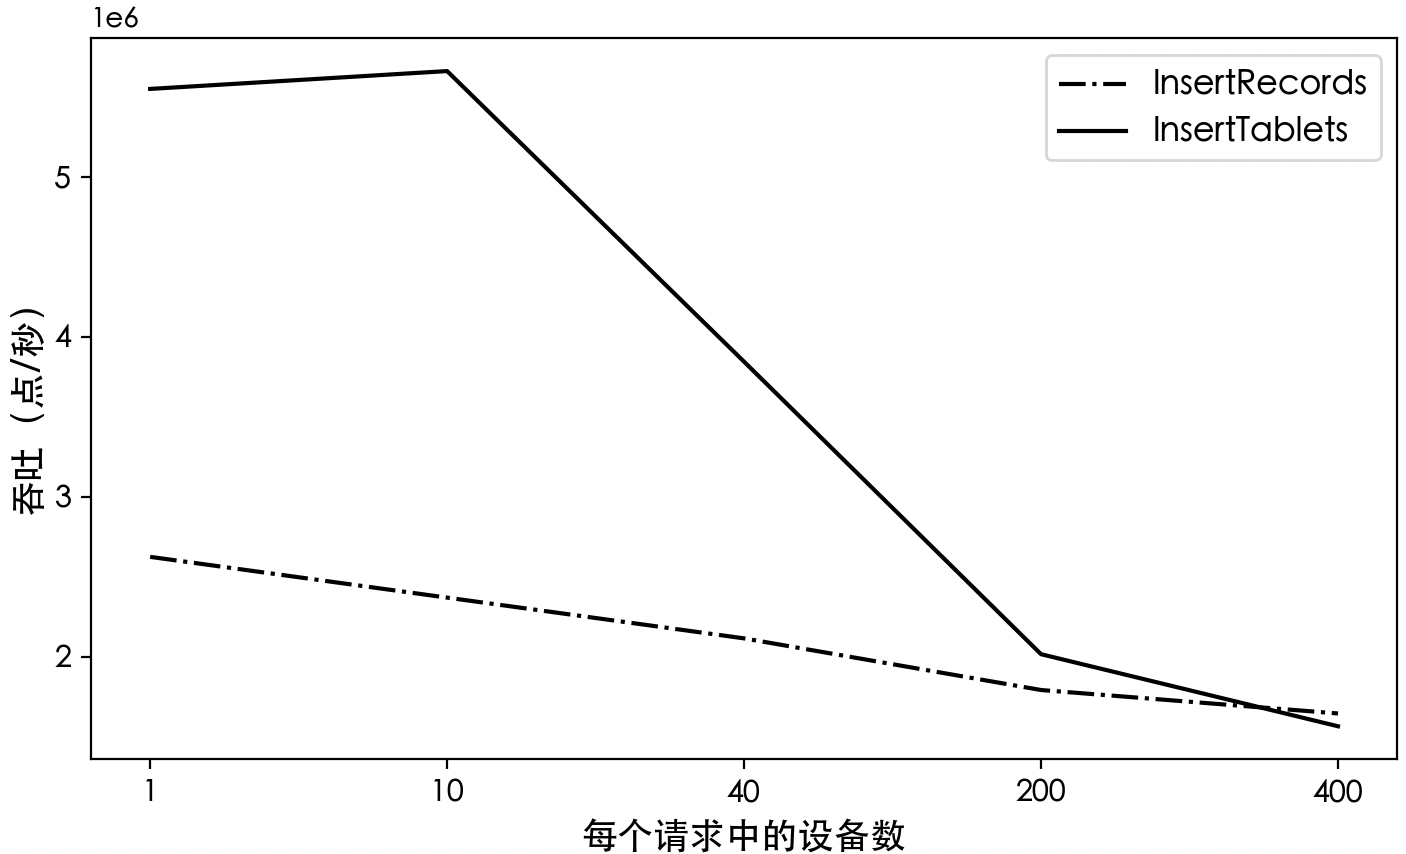
\includegraphics[width=0.8\linewidth]{records-vs-tablets-throughput.png}
  \caption{一次写入请求中写入吞吐随设备数的变化}
  \label{fig:records-vs-tablets-throughput}
\end{figure}

\begin{figure}
  \centering
  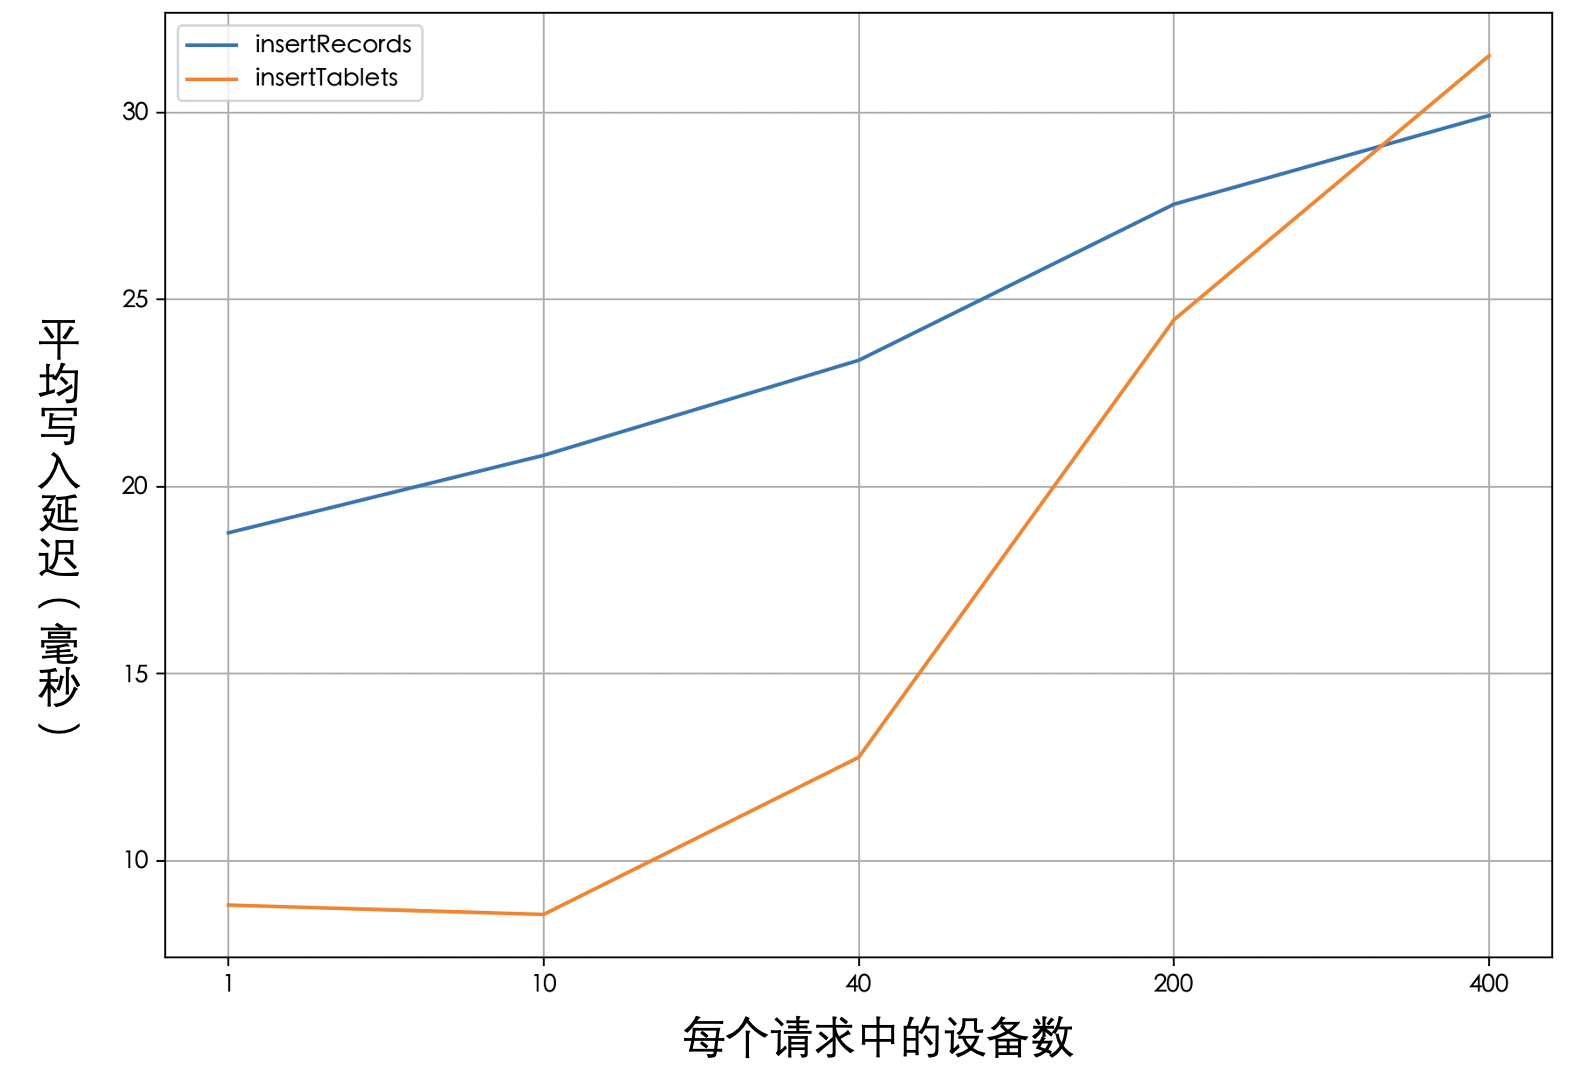
\includegraphics[width=0.8\linewidth]{records-vs-tablets-latency.png}
  \caption{一次写入请求中写入延迟随设备数的变化}
  \label{fig:records-vs-tablets-latency}
\end{figure}

从实验结果中可以看出,当设备数小于 400,即每个设备都有超过 1 条数据时,\emph{insertTablets} 接口的性能要优于 \emph{insertRecords};当设备数等于 400 时,也就是每个设备在一次请求中都只有 1 条数据时,\emph{insertRecords} 接口要略微优于 \emph{insertTablets}。这个实验结论与上一节中对这两个接口的分析是一致的,使用 Tablet 写入可以利用同一设备的数据被提前聚集的特点进行批量化写入,实现较好的性能;而 \emph{insertRecords} 由于提前不知道同一设备数据的分布,只能一条一条地写入存储引擎,性能较差。当一个请求中每个设备都只有一条数据时,使用 \emph{insertTablets} 接口写入时每个 Tablet 都只有一行数据,此时其执行逻辑实际上和 \emph{insertRecords} 是差不多的。由于 \emph{insertRecords} 针对行式写入有一些优化,因此其性能略好于 \emph{insertTablets}。


\subsection{不同接口的使用场景}
\emph{insertRecords} 和 \emph{insertTablets} 接口在设备和时间两个维度进行了批量化,而 \emph{insertTablet} 接口则时间这个维度进行了批量化。不同批量化维度会导致不同接口的适用场景有所不同。

按照数据产生的频率进行划分,可以将时序数据写入的场景分为高频和中低频两种场景。在高频场景中,传感器的采样率很高,短时间内会产生大量时序数据,并且这些数据都属于同一个设备。例如在风力发电场景中风机上的传感器在某些情况下的采样频率可以达到 8KHz\cite{李天安2020apache},如果将一个风机建模为一个设备,并且假设传感器的采样频率一致,那么一个设备每秒钟就会产生 8000 行数据。在中低频场景中,传感器的采样频率较低,可能每隔几十秒传感器才会产生一个数据点。例如在长安汽车的车联网场景中,一辆汽车被建模为一个设备,汽车上的传感器每隔 30 秒才会进行一次采样,如果所有传感器的采样频率一致,那么一个设备每隔 30 秒才会产生一行数据。

数据产生频率的不同会导致这些场景适用不同接口。在高频场景中,由于一个设备的数据产生地非常快,使用 \emph{insertTablet} 或者 \emph{insertTablets} 接口可以充分利用数据按设备批量化的特点,将其快速写入到存储引擎中。如果使用 \emph{insertRecords} 接口,则无法利用每个设备下数据较多的特点,将数据一行一行地写入,导致最终性能不高。在低频场景中,数据间隔很久才会产生,如果使用 \emph{insertTablet} 或者 \emph{insertTablets} 接口就有两种选择:
\begin{enumerate}
  \item 为了提高写入性能,对数据进行缓存和积攒,等到 Tablet 的大小较大时才写入。但是这样会导致数据从产生到写入会经历非常长的时间。以长安汽车为例,一辆汽车被建模为一个设备,假如需要积攒到一个 Tablet 中有 100 行数据才写入,那么数据从产生到写入数据库的延迟为 50 分钟,在此期间其他应用无法从数据库中查询到这些数据,这是不可接受的。
  \item 为了及时写入数据,在每个 Tablet 较小时就进行写入。从上一节的实验结果中我们可以知道这样不仅无法发挥出 Tablet 写入的性能,对数据分 Tablet 进行组装还会对上层应用带来额外的复杂度。
\end{enumerate}
如果使用 \emph{insertRecords},可以令 Record 的数量积攒到一定程度以后一起发送给服务器进行写入,并且 \emph{insertRecords} 的接口形式更加直观,可以减轻用户侧的复杂度。因此,长安汽车在其业务中选择的就是 \emph{insertRecords} 接口进行数据写入。

\begin{table}
  \centering
  \caption{不同写入接口的适用场景}
  \begin{tabular}{lll}
    \toprule
    接口 & 使用场景 & 原因 \\
    \midrule
    insertTablets & 单设备频率较高 & 写入性能最优\\
     insertRecords &  单设备频率较低,设备数较多 & 无需长时间积攒数据,延迟较低 \\
    \bottomrule
  \end{tabular}
  \label{tabular:insert-interfaces-scene}
\end{table}

但是,从 \ref{sec:chap3-sec1-1} 节中的实验结果不难发现,\emph{insertRecords} 接口虽然有着使用方便的优点,但是其性能与 \emph{insertTablets} 接口有一定的差距。因此,如果我们可以将 \emph{insertRecords} 写入接口的性能提升,那么对于用户而言既可以使用比较友好的接口,省去将数据归类为 Tablet 的繁琐过程,又可以获得不错的写入性能。所以,本文的研究重点是如何在保持 \emph{insertRecords} 接口不变的情况下,通过设计新的底层实现机制,实现高性能的 \emph{insertRecords} 写入。


\section{Apache IoTDB 中 \emph{insertRecords} 写入的实现\label{sec:chap3-sec2}}
在研究如何设计出新的 \emph{insertRecords} 写入实现机制之前,本文先介绍目前 Apache IoTDB 对 \emph{insertRecords} 写入机制的实现。从应用层调用 IoTDB SDK 提供的 \emph{insertRecords} 接口开始,写入会经历客户端侧的数据预处理、RPC 层数据序列化与反序列化、存储引擎侧数据写入内存表以及内存表数据的持久化。下面将详细介绍这个过程。
\subsection{客户端侧的数据预处理流程}
客户端在接收到用户传入的写入数据后,需要对数据进行语义校验、划分和封装,其操作如下:
\begin{itemize}
  \item \emph{insertRecords} 的每一个参数都是列表(List),在合法的语义下每个参数的长度应该相同,如果不同参数的列表长度不一致就需要停止写入并抛出错误。
  \item 经过校验之后,数据会进行分片。Apache IoTDB 是一个分布式的数据库,一个集群中可能存在多个数据节点。一条时间序列的数据会被切分成多片,分布在多个数据节点中\cite{wang2023apache}。用户通过接口传入的一批数据就可能需要写入不同的节点。为了更高效地写入,IoTDB 的客户端会缓存不同序列对应的数据节点地址,然后将传入的数据按照节点地址进行划分,写入同一个节点的数据集合成一个子请求。
  \item 每一个子请求都包含了用户写入的数据的若干行,包括这些行的设备 ID、时间序列 ID、数据类型、时间戳以及数据值。IoTDB 客户端在把数据交由 RPC 层进行传输前,会提前把数据类型以及数据值序列化为二进制数据。每一行序列化的格式都如图 \ref{fig:curr-line-serialize-format} 所示:首先序列化一个数据点的类型,然后是它的值,紧接着是下一个数据点的类型和值。一行数据序列化为一个字节流对象(ByteBuffer),一个请求中的多行数据序列化的结果是字节流对象的列表(List<ByteBuffer>),其中的每一个元素都代表了原来的一行数据。
\end{itemize}

\begin{figure}
  \centering
  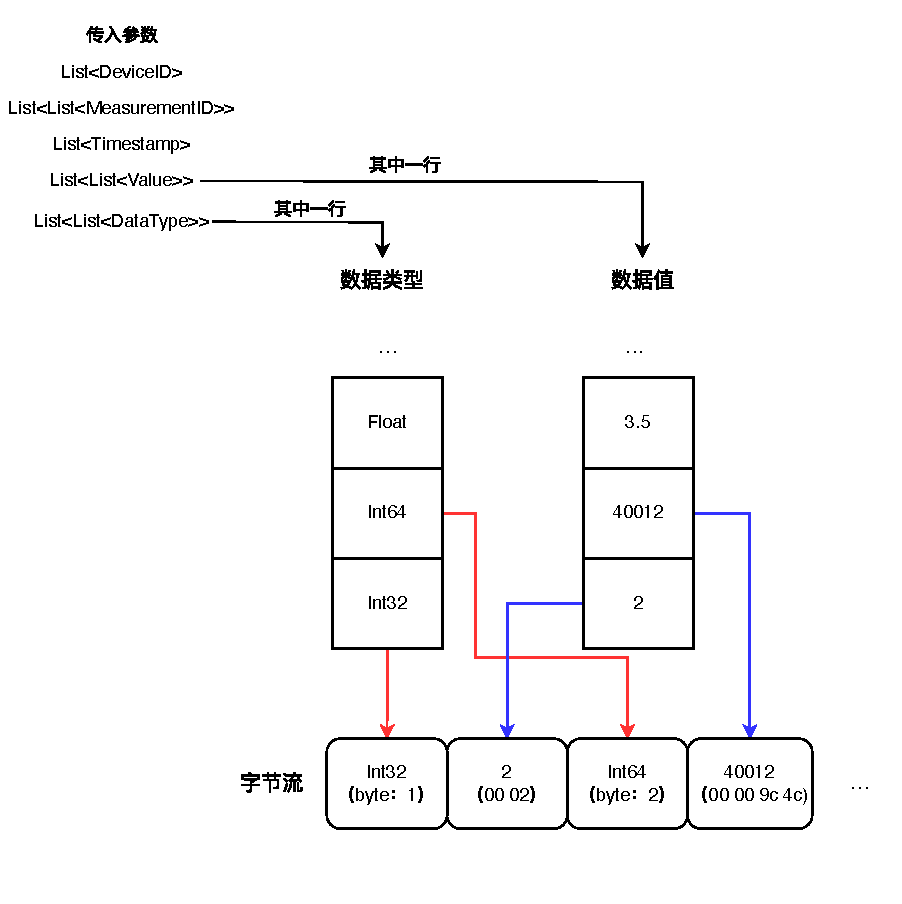
\includegraphics[width=0.8\linewidth]{curr-data-serialize.pdf}
  \caption{一行数据序列化过程}
  \label{fig:curr-line-serialize-format}
\end{figure}

经过以上步骤,客户端就完成了对待写入数据的语义校验、分片和序列化,然后将这些数据交由 RPC 层传输到服务器。
\subsection{RPC 层的数据序列化与反序列化流程}
Apache IoTDB 使用了 Apache Thrift\cite{apache2024thrift} 作为 RPC 层。Apache Thrift 是一个跨语言的 RPC 框架,它使得开发者可以在一个语言中编写服务器端应用程序,并且可以从其他语言编写的客户端进行通信,从而极大地简化了多语言开发的复杂性。

Thrift 的工作原理基于定义一个服务的接口描述语言(Interface Description Language, IDL)。开发者首先需要用 Thrift IDL 来定义数据类型和服务接口。然后,Thrift 编译器会自动为当前所使用的编程语言生成相应的代码,包括数据类型的定义、服务接口的框架以及序列化/反序列化的机制。下面分别介绍客户端侧与服务器侧 Thrift 传输和接收数据的过程。
\subsubsection{客户端侧序列化与传输数据流程\label{sec:chap3-sec2-2-1}}
下面以 Apache IoTDB 目前对 Thrift 的配置为例,介绍 Thrift 传输客户端将预处理好的 \emph{insertRecords} 数据的过程。

IoTDB 在 Thrift 中对 \emph{insertRecords} 接口的定义如下:
\begin{lstlisting}[language=idl,frame = trBL , firstnumber = last , escapeinside={(*@}{@*)}]
struct TSInsertRecordsReq {
  1: required i64 sessionId
  2: required list<string> deviceIds
  3: required list<list<string>> measurementsList
  4: required list<binary> valuesList
  5: required list<i64> timestamps
}

TSStatus insertRecords(1:TSInsertRecordsReq req);
\end{lstlisting}
TSInsertRecordsReq 结构体内部的数据对应了 \emph{insertRecords} 接口的参数,Thrift 会将客户端传下的参数封装为一个 TSInsertRecordsReq 实例。然后,Thrift 将封装好的 TSInsertRecordsReq 进行序列化。IoTDB 使用的是 Thrift 的 TBinaryProtocol,这是一种二进制数据通讯协议,将数据以字节流的形式传输,因此 Thrift 需要将 TSInsertRecordsReq 序列化为字节流,其流程如图 \ref{fig:thrift-serialize} 所示,每个步骤的详细操作如下:
\begin{enumerate}
  \item 写入消息开始的标志(writeMessageBegin):序列化该条 RPC 的元信息,包括 Thrift 的版本号、RPC 调用的方法名称、本条消息的 ID。
  \item 校验当前参数是否合法(validate):检查在 IDL 的定义中标记为 \emph{required} 的字段在传入的 TSInsertRecordsReq 结构体中是否被设置,如果没有则抛出错误,停止数据传输。
  \item 写入结构体开始的标志(writeStructBegin):在二进制数据传输协议中,这一步不会序列化数据。如果使用其他数据传输协议,例如 JSON 协议,就会写入结构体开始的标志,例如 JSON 的上下文和左括号。
  \item\label{item:write-field-begin}  序列化一个字段开始的标志(writeFieldBegin):在这一步中 Thrift 会记录该字段的 ID 和类型。
  \item 写入字段的内容(writeField):序列化一个字段的实际数据,Thrift 支持多种基础数据类型和复杂数据结构,在这一步中会将这些数据或数据结构根据其类型的不同使用不同的方式(如 writeI64、writeString、writeList 等)序列化为二进制的字节流。
  \item 写入字段结束(writeFieldEnd):在二进制传输协议中,这一步不会序列化数据。如果使用其他数据传输协议,例如 JSON 协议,就会写入上下文和 JSON 的右括号。在这一步结束之后,如果当前结构体还有字段没有序列化,就会返回第 \ref{item:write-field-begin} 步,否则进入到下一步。
  \item 写入结构体结束的标志(writeStructEnd):在二进制传输协议中,这一步不会序列化数据。如果使用其他数据传输协议,例如 JSON 协议,就会写入上下文和 JSON 的右括号。
  \item 写入消息结束的标记(writeMessageEnd):序列化该条消息结束的标志。
\end{enumerate}
\begin{figure}
  \centering
  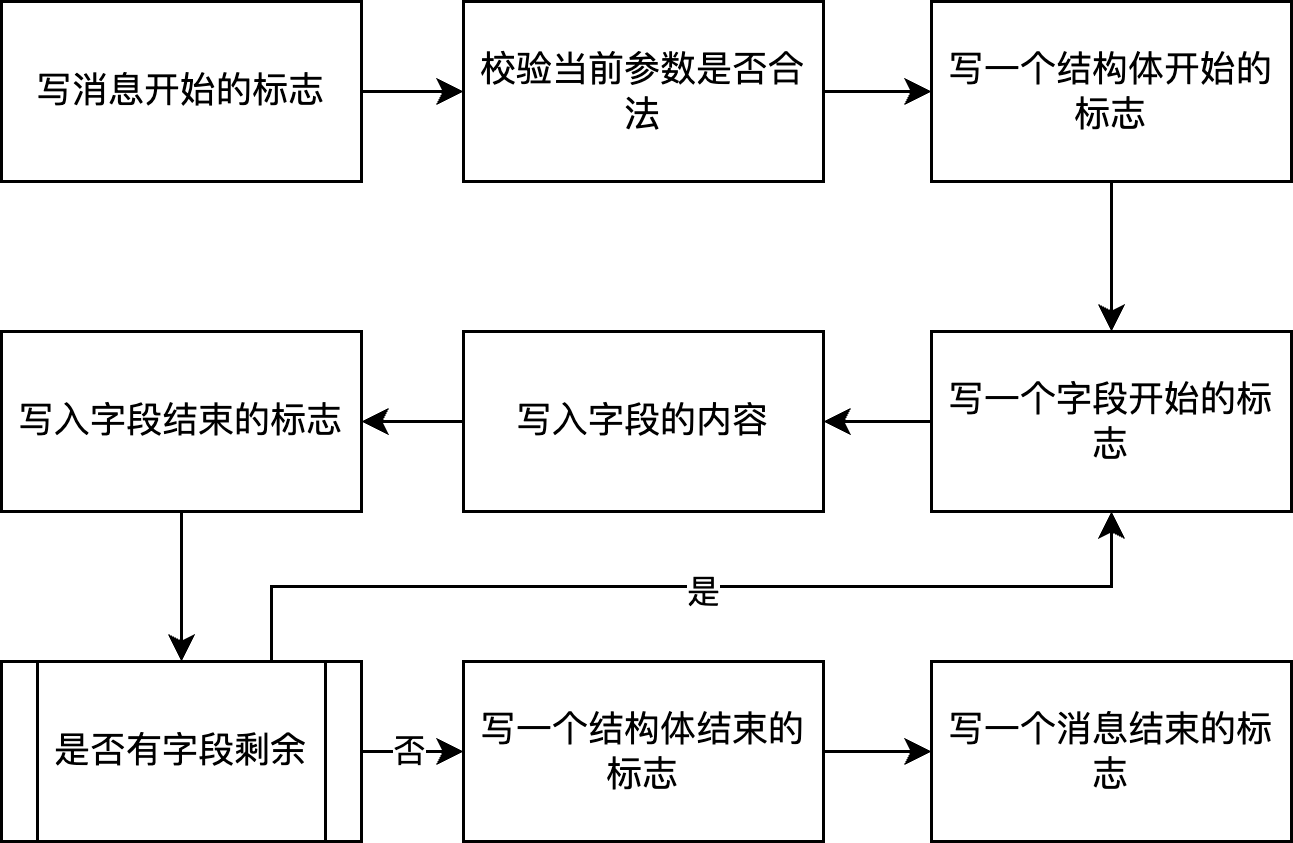
\includegraphics[width=0.9\linewidth]{thrift-serialize.png}
  \caption{Thrift 将请求结构体序列化为字节流的过程}
  \label{fig:thrift-serialize}
\end{figure}
经过以上步骤,Thrift 就将一个 TSInsertRecordsReq 结构体序列化为二进制数据了。然后将这些数据交由 Thrift 的传输层(TTransport)通过网络传输。IoTDB 对 Thrift 的 TTransport 进行了修改,实现了名为 TElasticFramedTransport 的传输层,其将传输协议传递下来的数据缓存到一个缓冲区(Buffer)中,等待一帧消息写完了之后再一起通过 Socket 传输到服务器。
\subsubsection{服务器侧接收与反序列化数据}
Thrift 首先从传输层(TElasticFramedTransport)接收一帧完整消息的字节数据,然后将这些数据进行反序列化。服务器端的反序列化过程是客户端序列化的逆过程,将数据从二进制的字节流还原为编程语言中的请求结构体,这个流程如图 \ref{fig:thrift-deserialize} 所示。
\begin{figure}
  \centering
  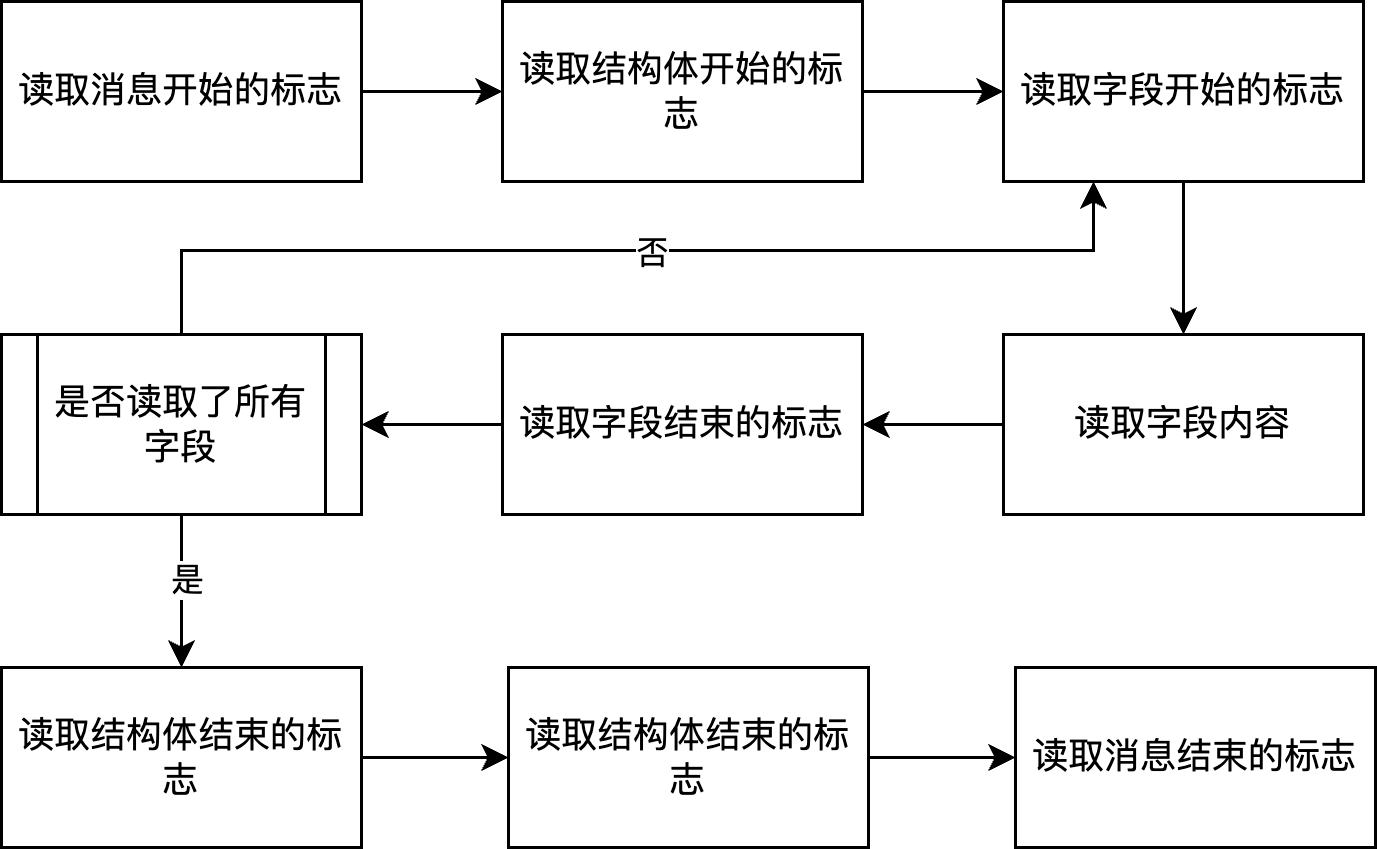
\includegraphics[width=0.9\linewidth]{thrift-deserialize.png}
  \caption{Thrift 将字节流数据反序列化为请求结构体的过程}
  \label{fig:thrift-deserialize}
\end{figure}

在反序列化的这些步骤中,最重要的是对一个结构体中每个字段的解析。Thrift 在客户端序列化数据时,保存了每个字段的 ID 和类型。在反序列化时,先读取到这个字段的 ID,然后读取到这个字段的类型,然后判断服务器段结构体的定义中该字段是否为该类型,如果是,则根据字段的类型选择不同反序列化方法(readI64、readString、readList)将这个字段的内容从字节流中还原出来。当所有字段都还原出来以后,Thrift 将这些字段封装为一个 TSInsertRecordsReq 结构体,并交由 IoTDB 进行下一步处理。
\subsection{IoTDB 写入存储引擎前的预处理}
IoTDB 在收到 RPC 层组装好的 TSInsertRecordsReq 结构体以后首先会进行一系列的预处理,然后才会交由存储引擎写入内存表中。这些预处理工作包括:
\begin{itemize}
  \item \textbf{时间序列 ID 校验}:对写入的时间序列 ID 进行检查,判断其是否符合 IoTDB 对时间序列 ID 的规定,例如不能包含系统的保留字,不能为未转义的纯数字等。值得注意的是,这一步是与 IoTDB 内部的信息无关的,也就是即使没有 IoTDB 中记录的用户数据也可以完成校验。
  \item \textbf{数据结构转换}:TSInsertRecordsReq 是 Thrift 中定义的一个数据结构,并不利于 IoTDB 的后续写入处理,所以在预处理步骤中 IoTDB 会将 TSInsertRecordsReq 转换为 InsertRowsStatement 这一数据结构。在这一过程中,还会将客户端侧序列化的每一行数据还原成 Java 中的数据结构。
  \item \textbf{权限检查}:检查当前用户是否具有对被写入时间序列都写入权限。
  \item \textbf{元数据校验与创建}:区别于前面的语法校验,这一步是与 IoTDB 的内部信息有关的。在这一步骤中,IoTDB 验证写入请求中的时间序列是否已经被创建。如果序列已经被创建,则验证当前写入请求中该时间序列的类型是否与之前创建的类型相符,如不符合就拒绝写入;如果没有创建且用户开启了元数据自动创建功能,就会创建该时间序列的元数据,否则拒绝写入。这个步骤中元数据信息可能不存在当前的 DataNode 节点中,有可能需要通过网络向别的 DataNode 节点拉取元数据信息。为了加速这一步骤,每个 DataNode 都维护了一个元数据的缓存,以减少通过网络获取元数据的次数。
  \item \textbf{获取数据分区信息}:在 IoTDB 中数据被分为多个 DataRegion,每个时间序列的一段数据会被分配到一个 DataRegion 中,不同的 DataRegion 可能处于同一个节点,也可能处于不同的节点。这一步骤计算写入请求中每一条时间序列所属的 DataRegion,并按照所属的 DataRegion 将它们分成多个写入计划片段(FragmentInstance),每个片段都包含了需要写入到一个 DataRegion 中的数据。
\end{itemize}
经过这些预处理之后,一个写入请求变成了一个或多个写入计划分片(FragmentInstance),这些 FragmentInstance 有些是写入到本节点的 DataRegion 中的,有些是写入到其他节点的 DataRegion 中的。对于写入到本节点 DataRegion 中的 FragmentInstance,会串行地交给存储引擎执行;对于写入到其他节点 DataRegion 的 FragmentInstance,则会并行地发送给其他节点执行。除此之外,为了能够对 IoTDB 的状态进行观测,以上的每一个步骤都会记录操作所需要的时间,然后记录到 IoTDB 的监控框架中。
\subsection{存储引擎侧数据写入内存表流程}
当存储引擎接收到一个 FragmentInstance 之后,首先会检查当前节点写前日志的大小是否超过了一定阈值(默认为 50GB),如果超过了就会阻塞当前写入线程。这么做的原因是,IoTDB 在分布式部署时使用 IoT Consensus 协议在不同节点间进行数据同步\cite{wang2023apache},数据同步时的每一条日志项就是写前日志的一个日志项。如果写前日志的体积很大,那么说明写入到该节点的数据未能及时同步到其他节点,IoTDB 通过阻塞写入来避免不同节点之间的数据差异进一步扩大。

然后,存储引擎会逐条写入待插入的记录。对于每一条记录,首先计算出该记录所属的时间分区(Time Partition),再判断该记录在该时间分区下是顺序数据还是乱序数据。这么做是因为 IoTDB 将一个 DataRegion 下的数据根据时间范围划分为多个时间分区,在每个时间分区内又将顺序数据和乱序数据分离存储,以提升系统的性能。IoTDB 为每个时间分区的顺序数据和乱序数据分别维护了一个内存表,前面的计算结束以后系统就决定了应该将这一行记录写到哪个内存表中。

在将数据写入到对应的内存表之前,系统还需要经过两个步骤:内存开销计算以及记录写前日志。为了避免系统在运行时发生内存不足(OutOfMemory,OOM)的情况,IoTDB 记录了每行写入数据的内存,并将这些内存开销同一记录。当使用的系统内存接近阈值时,就会挑选占有内存最多的内存表,将它们持久化到磁盘上,并释放对应的内存。对于每一行数据,系统会根据其中每个数据点的数据类型、长度等信息,计算出在内存中保存该行记录所需要的内存大小,然后记录到全局的内存管理器中。如果系统内存资源已经接近枯竭(默认为使用超过 90\%),则会阻塞当前写入,避免系统崩溃。

计算完内存开销以后,为了在 IoTDB 意外崩溃时仍能保证写入数据的持久性,系统为对每行写入的记录都保存一份写前日志(Write Ahead Log,WAL)。IoTDB 首先会将一行写入的记录作为写前日志项(WAL Entry)提交到写前日志序列化队列中,这个队列是一个大小有限的并发安全阻塞队列,队列的另一端有若干个线程将写前日志项序列化为字节流形式的写前日志,并缓存在内存的缓冲区(WAL Buffer)中。当缓冲区的大小超过了阈值(默认为 10MB),或者缓冲区中最旧的数据保持超过了一定的时间(默认为 500ms),就会将内存里的缓冲区持久化到磁盘上\cite{朱海铭2023面向内存表的可动态配置预写日志框架}。在一般情况下,写入线程不会等待内存中的 WAL Buffer 持久化后才进行下一步写入,但是如果写前日志项队列已经满了,那么写入线程就会被阻塞,直到队列前端的 WAL Entry 被序列化并腾出了空间给当前 WAL Entry,写入才会进行到后续的步骤。

当系统成功写完 WAL 以后,就可以将数据插入到内存表(MemTable)中了。IoTDB 的内存表抽象地看是一个两层嵌套的映射(Map):首先维护从设备 ID(Device ID)到数据块组(ChunkGroup)的映射,每个块组中又维护了时间序列 ID 到数据块(Chunk)的映射。一个数据块组保存了一个设备下的时间序列在内存中缓存的数据,一个数据块则保存了一条时间序列在内存中的数据。写入一行记录时,首先根据该行记录所属的设备找到对应的数据块组,然后把记录里每个数据点分别写入其所属的数据块中,其流程如图 \ref{fig:fragment-instance-insert-to-memtable} 所示。

\begin{figure}
  \centering
  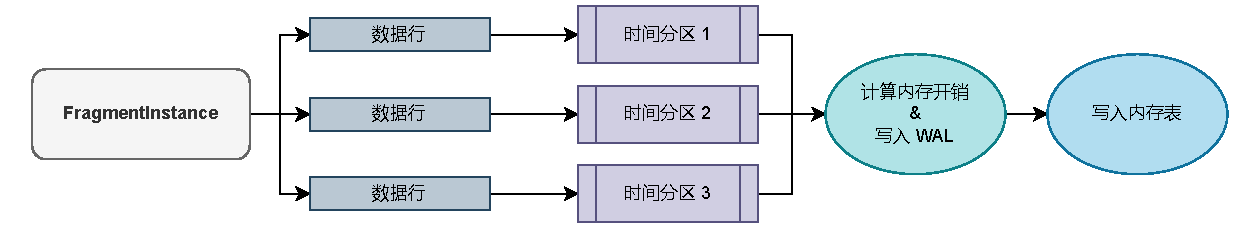
\includegraphics[width=\linewidth]{FragmentInstance写入MemTable流程.pdf}
  \caption{Fragment Instance 写入内存表过程}
  \label{fig:fragment-instance-insert-to-memtable}
\end{figure}

至此,内存已经保存在了 IoTDB 中。IoTDB 中为了提升查询性能,维护了一些数据缓存以及文件的内存索引。在数据写入内存表后,系统还需要更新数据缓存和文件的内存索引。同时,系统也会记录写入过程中的一系列时间开销,例如记录 WAL 的耗时、写入内存表的耗时等,并将这些统计出来的耗时记录到 IoTDB 的内存框架中。
\subsection{存储引擎侧数据持久化流程}
当 IoTDB 的内存表占据的内存到达一定阈值以后,系统就会把内存表持久化到磁盘上,这个过程成为刷盘(Flush)。IoTDB 内存表中刷盘的最基本单位是数据块,也就是一条时间序列在内存中所对应的数据。一个内存数据块会经过编码(Encode)、压缩(Compress)和 I/O 三个阶段的处理最终成为磁盘上的一个数据块,如图 \ref{fig:memtable-flush} 这三个过程是异步的过程,互相之间以生产者-消费者模式(Producer-Consumer Pattern)连接。为了在查询时快速定位到磁盘文件的数据块,系统会在每个文件的尾部构建一个当前文件的数据索引。当一个内存表中的所有数据都持久到了磁盘上以后,该内存表占据的内存就会被释放,系统就有了空闲的内存处理新的写入请求。

\begin{figure}
  \centering
  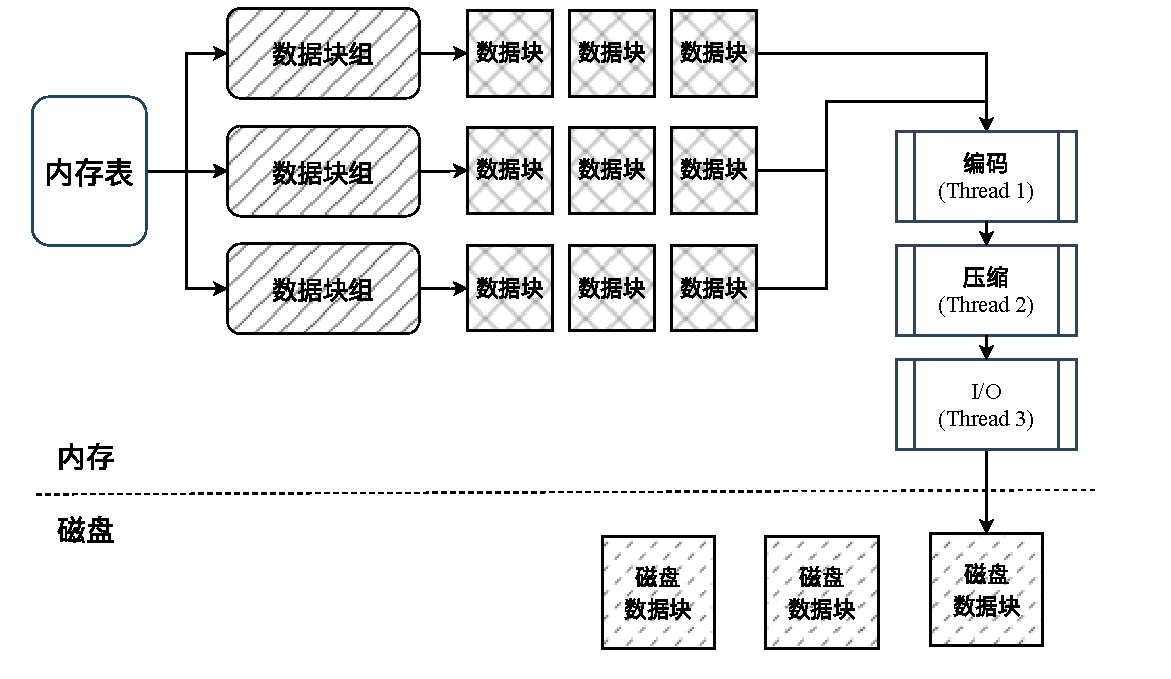
\includegraphics[width=\linewidth]{IoTDB刷盘过程.pdf}
  \caption{内存表持久化过程}
  \label{fig:memtable-flush}
\end{figure}

\section{当前机制性能分析}
\subsection{实验与结果分析\label{sec:chap3-sec3-1}}
在 \ref{sec:chap3-sec2} 节中,本文介绍了 IoTDB 目前的 \emph{insertRecords} 写入机制。从 \ref{sec:chap3-sec1-1} 节的实验中,本文发现在单个写入请求中,如果每个设备的写入行数大于 1 时,通过 \emph{insertRecords} 接口写入的吞吐和延迟均不如 \emph{insertTablets}。本节将使用 Arthas 工具对使用 \emph{insertRecords} 和 \emph{insertTablets} 接口写入的 IoTDB 进行抽样(Profiling),并结合 IoTDB 监控框架所采集到的数据,分析当前 \emph{insertRecords} 性能较差的原因。


IoTDB 所使用的配置如表 \ref{tabular:insert-records-profile-iotdb-config} 所示,测试使用的写入工具为 IoT Benchmark\cite{liu2019benchmarking},其配置如表 \ref{tabular:insert-records-profile-benchmark-config} 所示。使用 Arthas 对 IoTDB 写入过程中各个阶段的 CPU 开销抽样的结果如表 \ref{tabular:insert-records-profile-result} 所示,其中的加粗的阶段是本工作后续部分进行优化的部分。

从性能分析的结果对比中不难发现,使用 \emph{insertRecords} 写入时,时间序列 ID 检验、元数据校验、计算内存开销、记录写前日志、维护缓存与内存索引以及写入监控信息这几个步骤相较于 \emph{insertTablets} 中的占据的比例都显著更高。从前文的 \emph{insertRecords} 的机制分析中可以推测出这个现象的原因:无论是在预处理阶段还是执行阶段,\emph{insertTablets} 都是一整个 Tablet 一起执行的,一个 Tablet 只需要预处理和写入一次;而 \emph{insertRecords} 是一行行地执行的,每一行数据都要预处理和写入一次。然而,无论是一行还是一个 Tablet,校验一次时间序列 ID、更新一次监控数值、维护一次缓存等的代价都是相同的,而 \emph{insertRecords} 调用这些组件的次数更多,最终造成在这个测试场景中虽然写入的数据量相同,但是 \emph{insertRecords} 的开销比 \emph{insertTablets} 更大,性能也更低。为了避免这样的现象,新的 \emph{insertRecords} 写入机制在存储引擎侧执行时,应该最大程度地进行批量化执行。
\begin{table}
  \caption{IoT Benchmark 测试配置表}
  \centering
  \begin{tabular}{ll}
  \toprule
  配置名称 & 配置描述 \\
  \midrule
      写入设备数 &  50000 \\ 
      每个设备下的时间序列数 & 20 \\ 
      存储组数量 & 10 \\ 
      并发写入客户端数 & 25 \\ 
      单个请求的数据总行数 &  1000 \\ 
      操作系统 & Ubuntu 20.04.2 LTS,64位 \\
      JDK 版本 & OpenJDK 11.0.22 \\
  \bottomrule
  \end{tabular}
  \label{tabular:insert-records-profile-benchmark-config}
\end{table}

\begin{table}
  \caption{IoTDB 测试配置表}
  \centering
  \begin{tabular}{ll}
  \toprule
  配置名称 & 配置描述 \\
  \midrule
      IoTDB 版本 &  1.1.0 \\ 
      DataNode 内存 & 28 GB \\ 
      ConfigNode 内存 & 2GB \\ 
      IoTDB 部署方式 & 1 ConfigNode + 1 DataNode \\
      JDK 版本 & OpenJDK 11.0.22 \\
      操作系统 & Ubuntu 20.04.2 LTS,64位 \\
      CPU &  Intel I7-11700,8 核 16 线程 \\ 
      硬盘 & HDD(希捷 ST-16000NM000J) \\ 
      网络环境 & 1000 Mbps 局域网 \\
  \bottomrule
  \end{tabular}
  \label{tabular:insert-records-profile-iotdb-config}
\end{table}

\begin{table}
  \caption{写入各阶段 CPU 占用}
  \centering
  \begin{tabular}{lll}
  \toprule
  阶段 &  \emph{insertRecords} & \emph{insertTablets} \\
  \midrule
      \textbf{Thrift 反序列化} &  14.14\% & 13.20\% \\ 
      \textbf{时间序列 ID 检验} & 17.55\% & 1.38\% \\ 
      数据结构转换 &  8.65\% & 43.84\% \\ 
       权限检查 & 0.00\%(非常低,可忽略) &  1.22\%\\ 
      元数据校验 &  6.66\% & 1.78\% \\ 
      获取数据分区信息 &  0.97\% & 3.72\% \\
      计算数据分区与顺乱序 &  0.72\%&  0.73\%  \\
      \textbf{计算内存开销} & 5.47\% & 0.55\% \\
      \textbf{记录写前日志} & 3.36\% & 0.81\%\\
      \textbf{写入内存表} & 12.60\% & 22.93\% \\
      \textbf{维护缓存与内存索引} & 10.83\% & 3.72\% \\
      \textbf{记录写入中的监控信息} & 19.20\% & 1.13\%\\
  \bottomrule
  % 60.1% vs 12.34%
  \end{tabular}
  \label{tabular:insert-records-profile-result}
\end{table}

表 \ref{tabular:wal-vs-tsfile-size} 记录了在上述 IoTDB 和 IoT Benchmark 配置下,使用 \emph{insertTablets} 接口和 \emph{insertRecords} 接口写入 20 分钟以后 IoTDB 向磁盘写入的 TsFile 总大小和写前日志总大小。在运行同样时间的写入后,使用 \emph{insertRecords} 接口不仅比使用 \emph{insertTablets} 接口写入的数据更多,产生的写前日志体积也更小。更多的写前日志意味着系统宝贵的 I/O 资源和内存资源中有相当大一部分被 WAL 占用了,从而导致系统的写入性能下滑。此外,当 WAL 体积过大,导致系统的 I/O 资源紧张无法将 WAL 及时写到磁盘上时,根据前文中所展示的 \emph{insertRecords} 写入流程,写入线程就有可能在向写前日志项队列提交任务时被阻塞,进一步降低了系统的性能。


\begin{table}
  \caption{使用两种接口写入 20 分钟后 TsFile 大小和 WAL 大小}
  \centering
  \begin{tabular}{llll}
  \toprule 
  接口 & 写入 WAL 总大小 & 写入 TsFile 总大小 & 二者比例 \\
  \midrule 
  \emph{insertTablets} &  70 GB & 34 GB &  2.05 \\
  \emph{insertRecords} & 178 GB & 25 GB & 7.12 \\
  \bottomrule
  \end{tabular}
  \label{tabular:wal-vs-tsfile-size}
\end{table}


\begin{figure}
  \centering
  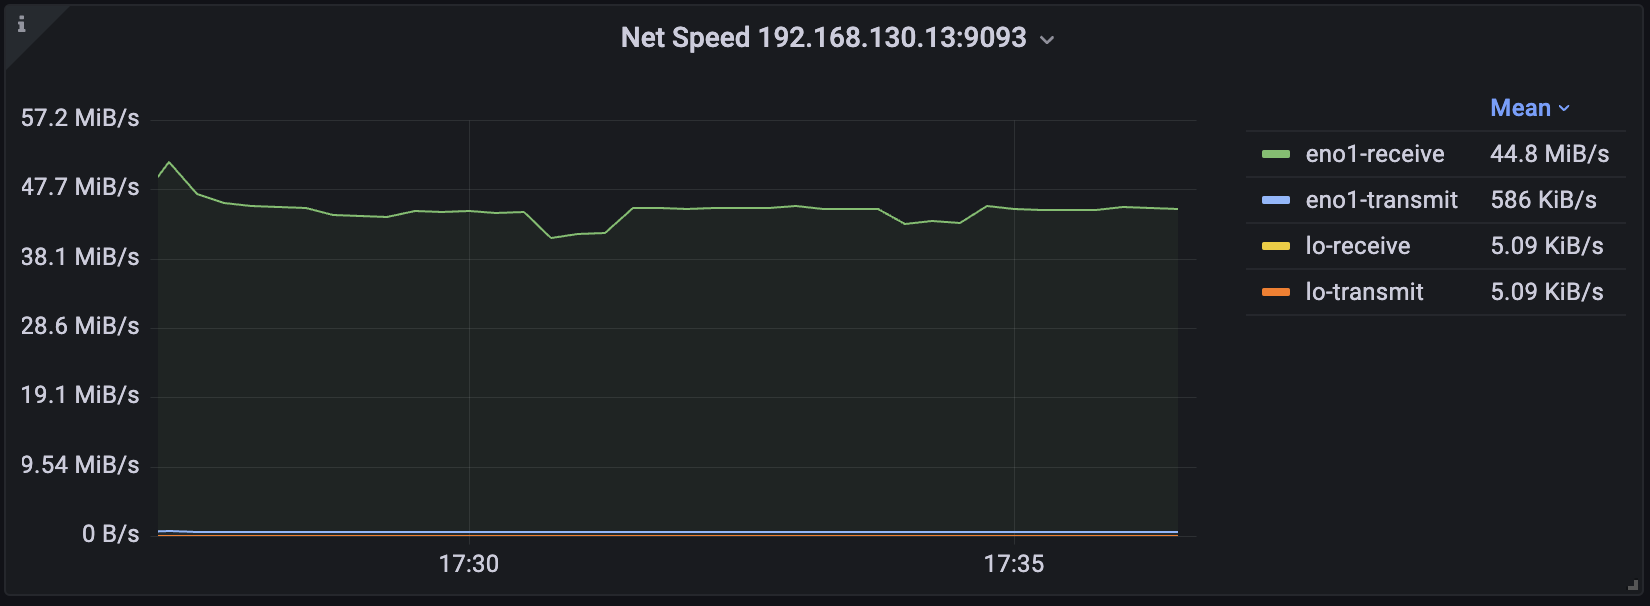
\includegraphics[width=\linewidth]{insertTablets-net.png}
  \caption{使用 \emph{InsertTablets} 接口写入时网络资源使用情况}
  \label{fig:curr-insert-tablets-net}
\end{figure}

\begin{figure}
  \centering
  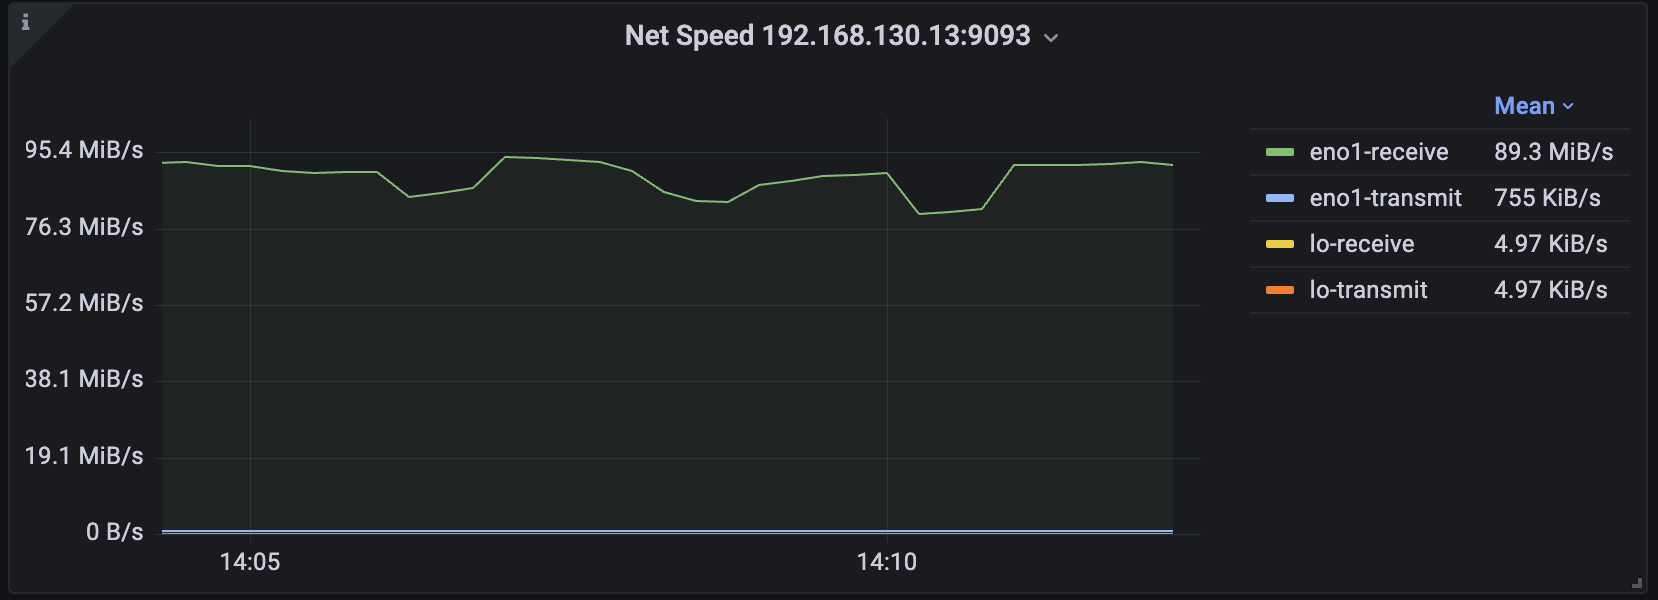
\includegraphics[width=\linewidth]{insertRecords-net.png}
  \caption{使用 \emph{insertRecords} 接口写入时网络资源使用情况}
  \label{fig:curr-insert-records-net}
\end{figure}



图 \ref{fig:curr-insert-tablets-net} 和图 \ref{fig:curr-insert-records-net} 展示了在进行上述实验时,IoTDB 监控框架所记录的网络资源使用情况。使用 \emph{insertRecords} 接口进行写入时,尽管实际写入的吞吐更少,但是系统所消耗的网络带宽却是使用 \emph{insertTablets} 接口的两倍,并且已经接近系统网络理论带宽的上限。根据前文中对客户端侧数据预处理和 RPC 层网络传输流程的介绍,导致这个现象的原因是 \emph{insertRecords} 在对写入请求进行序列化时,重复序列化了大量的数据(例如同一个设备的多行 Record,都会记录一遍该设备的 ID),导致包含同样数据的 \emph{insertRecords} 请求和 \emph{insertTablets} 请求,前者序列化得到的字节流比后者要更大。

\subsection{当前机制问题小结}
总结 \ref{sec:chap3-sec3-1} 节中的实验与分析,当前 \emph{insertRecords} 实现机制存在以下问题:
\begin{itemize}
  \item 服务器端对写入请求并非批量化执行,导致非核心流程占用了过多的资源,降低了写入效率;
  \item 相比于 \emph{insertTablets} 接口,\emph{insertRecords} 接口写入数据的 WAL 与 TsFile 比例过大;
  \item 相比于 \emph{insertTablets} 接口,\emph{insertRecords} 接口的写入请求序列化以后较为臃肿,占用了较多的网络资源。
\end{itemize}

\section{优化设计总览}
\begin{figure}
  \centering
  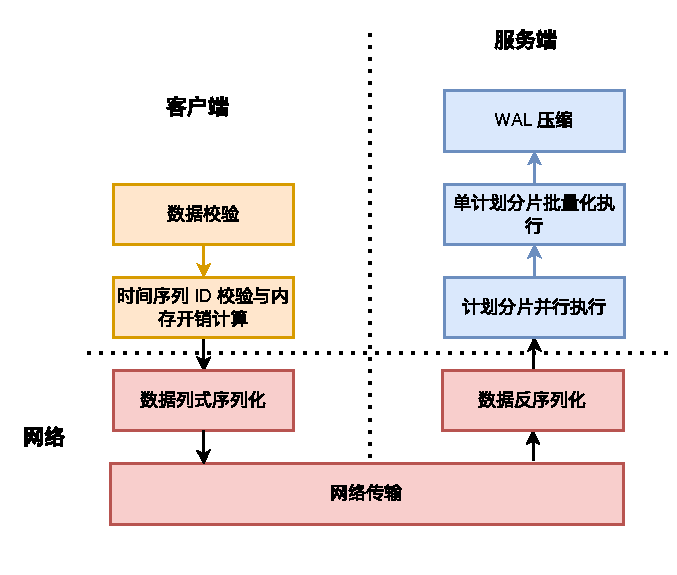
\includegraphics[width=\linewidth]{new-insert-records-overview.pdf}
  \caption{新 \emph{insertRecords} 写入机制}
  \label{fig:new-insert-records-overview}
\end{figure}

图 \ref{fig:new-insert-records-overview} 展示了新 \emph{insertRecords} 写入机制的总体设计。新写入机制有如下的设计目标:
\begin{enumerate}
  \item 提高系统性能:在相同的硬件下实现更高的写入性能,包括更高的吞吐以及更低的延迟;或者在相同的写入性能下降低对系统资源的使用;
  \item 提高系统整体资源的利用率:充分利用系统中客户端和服务器侧的计算、存储、网络资源,避免资源闲置;
  \item 具有高稳定性:在持续的高负载下系统应当能够保持较好的写入性能,避免出现剧烈的波动。
\end{enumerate}
为了实现这样的目标,新写入机制的总体设计思路为:
\begin{itemize}
  \item 存储引擎侧构建高效率的写入方式,将数据批量化、并行化写入,将写入过程中的固定开销尽量平摊到多条数据上,提高系统资源的利用率。
  \item 将服务器端的部分工作卸载(Offload)到客户端上,在客户端侧进行少量轻量级的计算,提高整体资源的利用率。
  \item 减少经过网络传输的冗余数据量,通过高效的列式数据格式提高网络资源的利用率。
\end{itemize}
本章的剩余内容从客户端、RPC 层、存储引擎三个方面简要介绍新 \emph{insertRecords} 写入机制的设计。

\section{客户端侧数据预处理}
在 \ref{sec:chap2-sec3} 节中,本文介绍了一些对于客户端进行优化的相关工作。其中, Crystal 存储系统基于远程存储所设计\cite{durner2021crystal}。因为数据通过远程存储设施进行读取的性能较差,所以为了提高系统的性能,Crystal 的客户端增加了谓词下推功能,被下推到数据源的谓词可以提前过滤掉一些不符合条件的数据,减少通过网络传输的数据量,提高系统的性能。在时序数据库中,TDEngine 的客户端也是“重客户端”设计的代表。TDEngine 的客户端不仅承担了对 SQL 进行解析的工作,还负责缓冲系统的元数据,在写入之前进行元数据校验。

目前 IoTDB 的客户端只负责数据的简单校验和传输,其余工作都由服务器承担。从系统的整体资源利用率的角度看,在目前的设计中 IoTDB 客户端侧的资源并没有被充分利用起来。因此,本文将服务器所承担的部分不依赖于已有数据的工作卸载到客户端侧。参考表 \ref{tabular:insert-records-profile-result} 可知,这一类工作中开销最大的就是时间序列 ID 和内存开销计算,本工作将会把这两项任务从服务器端移到客户端。

\section{写入请求列式序列化}
IoTDB 是一个时序数据库,本质上是一个针对时序场景优化的 OLAP 数据库\cite{谭新宇2023一致性协议}。在 OLAP 数据库中提高系统性能的一个常见方式是将数据按照列的形式存储和处理。根据 \ref{sec:chap3-sec2} 的对目前 IoTDB \emph{insertRecords} 写入请求序列化的介绍可以知道,目前所使用的序列化方式是行式的。结合 \ref{sec:chap3-sec3-1} 节的实验结果,可以得出目前行式序列化出来的写入请求较大,进而导致在实验环境下网络资源紧张的结论。为了解决这一问题,设计一个列式的数据序列化格式,并结合列式存储中常用的编码(Encode)、压缩(Compress)等技术,降低写入请求序列化后的体积。

正如 \ref{sec:chap2-sec3} 节中所述,设计序列化格式是一个需要权衡的过程,追求过小的数据包体积可能导致序列化和反序列化的开销过大,追求较低的序列化和反序列化开销则可能导致序列化得到的数据包体积过大。此外,由于 IoTDB 使用 Java 编写,数据序列化和反序列化对内存垃圾回收(Garbage Collection,GC)造成的影响也是我们需要考虑的重要因素。为了兼顾以上的因素,本文实现了一种可以根据系统当前负载状况动态使用压缩与编码的写入请求序列化方法。

\section{存储引擎侧批量并行化写入}
数据库系统高性能写入的实现离不开高性能存储引擎的支持。结合 \ref{sec:chap3-sec2} 节与 \ref{sec:chap3-sec3-1} 节的内容,IoTDB 存储引擎对 \emph{insertRecords} 写入实现最大的缺陷是没有做到批量化执行,造成了一些非核心流程的开销过大。因此,新 \emph{insertRecords} 写入机制在存储引擎侧执行写入请求时会将多条记录一齐写入到内存表中,在写入的过程中集中序列化写前日志、更新内存缓存、记录系统监控,避免多次调用这些非核心流程,通过统一调用来将它们的开销平摊到多条记录上。

以上的批量化写入是在计划分片(FragmentInstance,FI)级别的,而在 \ref{sec:chap3-sec2} 节的写入流程中,写入本地多个 DataRegion 的计划分片是串行执行的。当系统的负载不高时,这样串行执行并不能充分利用系统的资源。并且,由于后续分片的执行需要等待前序分片都执行完毕了才可以开始,写入的延迟也会提高。所以,本文将写入本地分片的过程并行化,以充分利用服务器多 CPU 核心的潜力。

在 \ref{sec:chap3-sec3-1} 节的实验结果中,\emph{insertRecords} 写入所产生的写前日志体积超过了最终 TsFile 体积的 7 倍,这不是一种合理的现象,大量的写前日志会占据系统的 I/O、内存和 CPU 资源。为了解决这一现象,新 \emph{insertRecords} 写入机制对写入同一 DataRegion 下的记录集中序列化写前日志,并且对写前日志采用轻量化的压缩算法进行压缩,显著地减少了写前日志的大小。


\section{本章小结}
本章首先介绍了 Apache IoTDB 中已有的写入接口,并对它们进行了性能和使用场景上的对比,说明了提高 \emph{insertRecords} 接口性能的意义。然后本章介绍了 Apache IoTDB 目前对 \emph{insertRecords} 写入机制的实现,并结合实验与性能分析,说明了目前 \emph{insertRecords} 写入机制存在的问题。随后,本章简要介绍了新 \emph{insertRecords} 写入机制的设计目标与设计思路,以及对客户端、RPC 层、存储引擎的设计要点,让读者从全局的视角了解本文的优化工作。后文将分别从客户端、RPC 层以及存储引擎三个角度深入地介绍每一项优化工作。

